\documentclass[pdf]{beamer}
\mode<presentation>{}

\usetheme{Frankfurt}
\usepackage{listings}
\usepackage{color}
\usepackage{amsmath}
\usepackage{wasysym}

\usefonttheme[onlymath]{serif}

%% preamble
\title[Random Forests]{CART, Bagging, and Random Forests}

\author{Paul Stey}
\date{Jan 12, 2017}

\begin{document}

%% title frame
\begin{frame}
\titlepage
\end{frame}



\begin{frame}<beamer>{Table of Contents}
	\tableofcontents[currentsection, 
				 currentsubsection, 
				 sectionstyle=show, 
				 subsectionstyle=show]
\end{frame}


\section{Introduction}
	\subsection{Trees}
		\begin{frame}{Species of Tree-Based Models}
			\begin{enumerate}
				\item ID3 (Quinlan, 1986)
				\item C4.5 (Quinlan, 1993)
				\item C5.0 (Quinlan, 1996)
				\item CART (Breiman, Friedman, Olshen, \& Stone, 1984)

			\end{enumerate}
		\end{frame}
			
	
		
		
	\subsection{CART}
	
				
		\begin{frame}{CART Pseudocode}
		\begin{enumerate}[]
			{\fontfamily{cmr}\selectfont
						
			\item $X$: matrix of predictors
			%\item $p$: number of columns in $X$
			\item $l$: current minimum loss at a given node
			\item $j^*$: index of column in $X$ that is current best predictor  
			
			\vspace{5 mm}			
			\item Pseudocode for \texttt{cart()} function:  
			\vspace{3 mm}

			\item{\textbf{while} number rows $>$ minimum-node-size}
				\item \hspace{3 mm} \textbf{for} $j = 1:p$
					\begin{enumerate}[  ]
						\item \hspace{6 mm} Find threshold, $t$, of $X_j$ that best partitions data
						\item \hspace{6 mm} If $t$ of $X_j$ produces loss $< l$, $X_j$ is current best predictor
						\item \hspace{6 mm} We update $l$ and $j^*$
					\end{enumerate}
				\item \hspace{3 mm} \textbf{end}
				\item \hspace{3 mm} Split data according to whether $X_{ij^*} < t$
				\item \hspace{3 mm} Call \texttt{cart()} on both partitions seperately
			\item \textbf{end}
			}
		\end{enumerate}
		\end{frame}
		
		\begin{frame}{Classification and Regression Trees}
			\begin{enumerate}
				\item Breiman \textit{et al.} (1984)
				\item Tree built by recursive binary splits 
				\item For regression, choose split that minimizes MSE
				\item For classification, choose splits by minimizing node impurity (e.g., Gini index) \\
				\begin{center}
					$$\sum_{k = 1}^{K} \hat{p}_{mk}(1 - \hat{p}_{mk})$$
				\end{center}
				where \\
				\begin{center}
					$$ \hat{p}_{mk} = \frac{1}{N_m} \sum_{x_i \in R_m} I(y_i = k)$$
				\end{center}
				is proportion of class $k$ observations in node $m$		
			\end{enumerate}
		\end{frame}

		
		\begin{frame}{Titanic Example}
			\begin{enumerate}
				\item Titantic data
				\item Kaggle competition
				\item Predicting survival (2-class problem)
				\item Using demographic and other variables
			\end{enumerate}
		\end{frame}
		
		
		
		\begin{frame}{Titanic Data}
		\begin{table}
		\begin{tabular}{l c c c c c c}
			\hline
			survived & age & sex & pclass & fare & sibsp & parch \\
			\hline
			1 	& 29.00 	& female	& 1	& 211.34	& 0	& 0 \\
			1 	& 0.92 	& male	& 1	& 151.55	& 1	& 2 \\
			0	& 2.00	& female	& 1	& 151.55	& 1	& 2 \\
			0 	& 30.00 	& male	& 1	& 151.55	& 1	& 2 \\
			0	& 25.00	& female	& 1	& 151.55	& 1	& 2 \\
			1 	& 48.00 	& male	& 1	& 151.55	& 0	& 0 \\
			1	& 63.00	& female	& 1	& 26.55	& 1	& 0 \\
			0	& 39.00	& male	& 1	& 0.00	& 0	& 0 \\
			1 	& 53.00 	& female	& 1	& 51.48	& 2	& 0 \\
			\hline
		\end{tabular}
		\end{table}
		\end{frame}
		
		
		\begin{frame}{Titanic Survial}
			\begin{figure}
				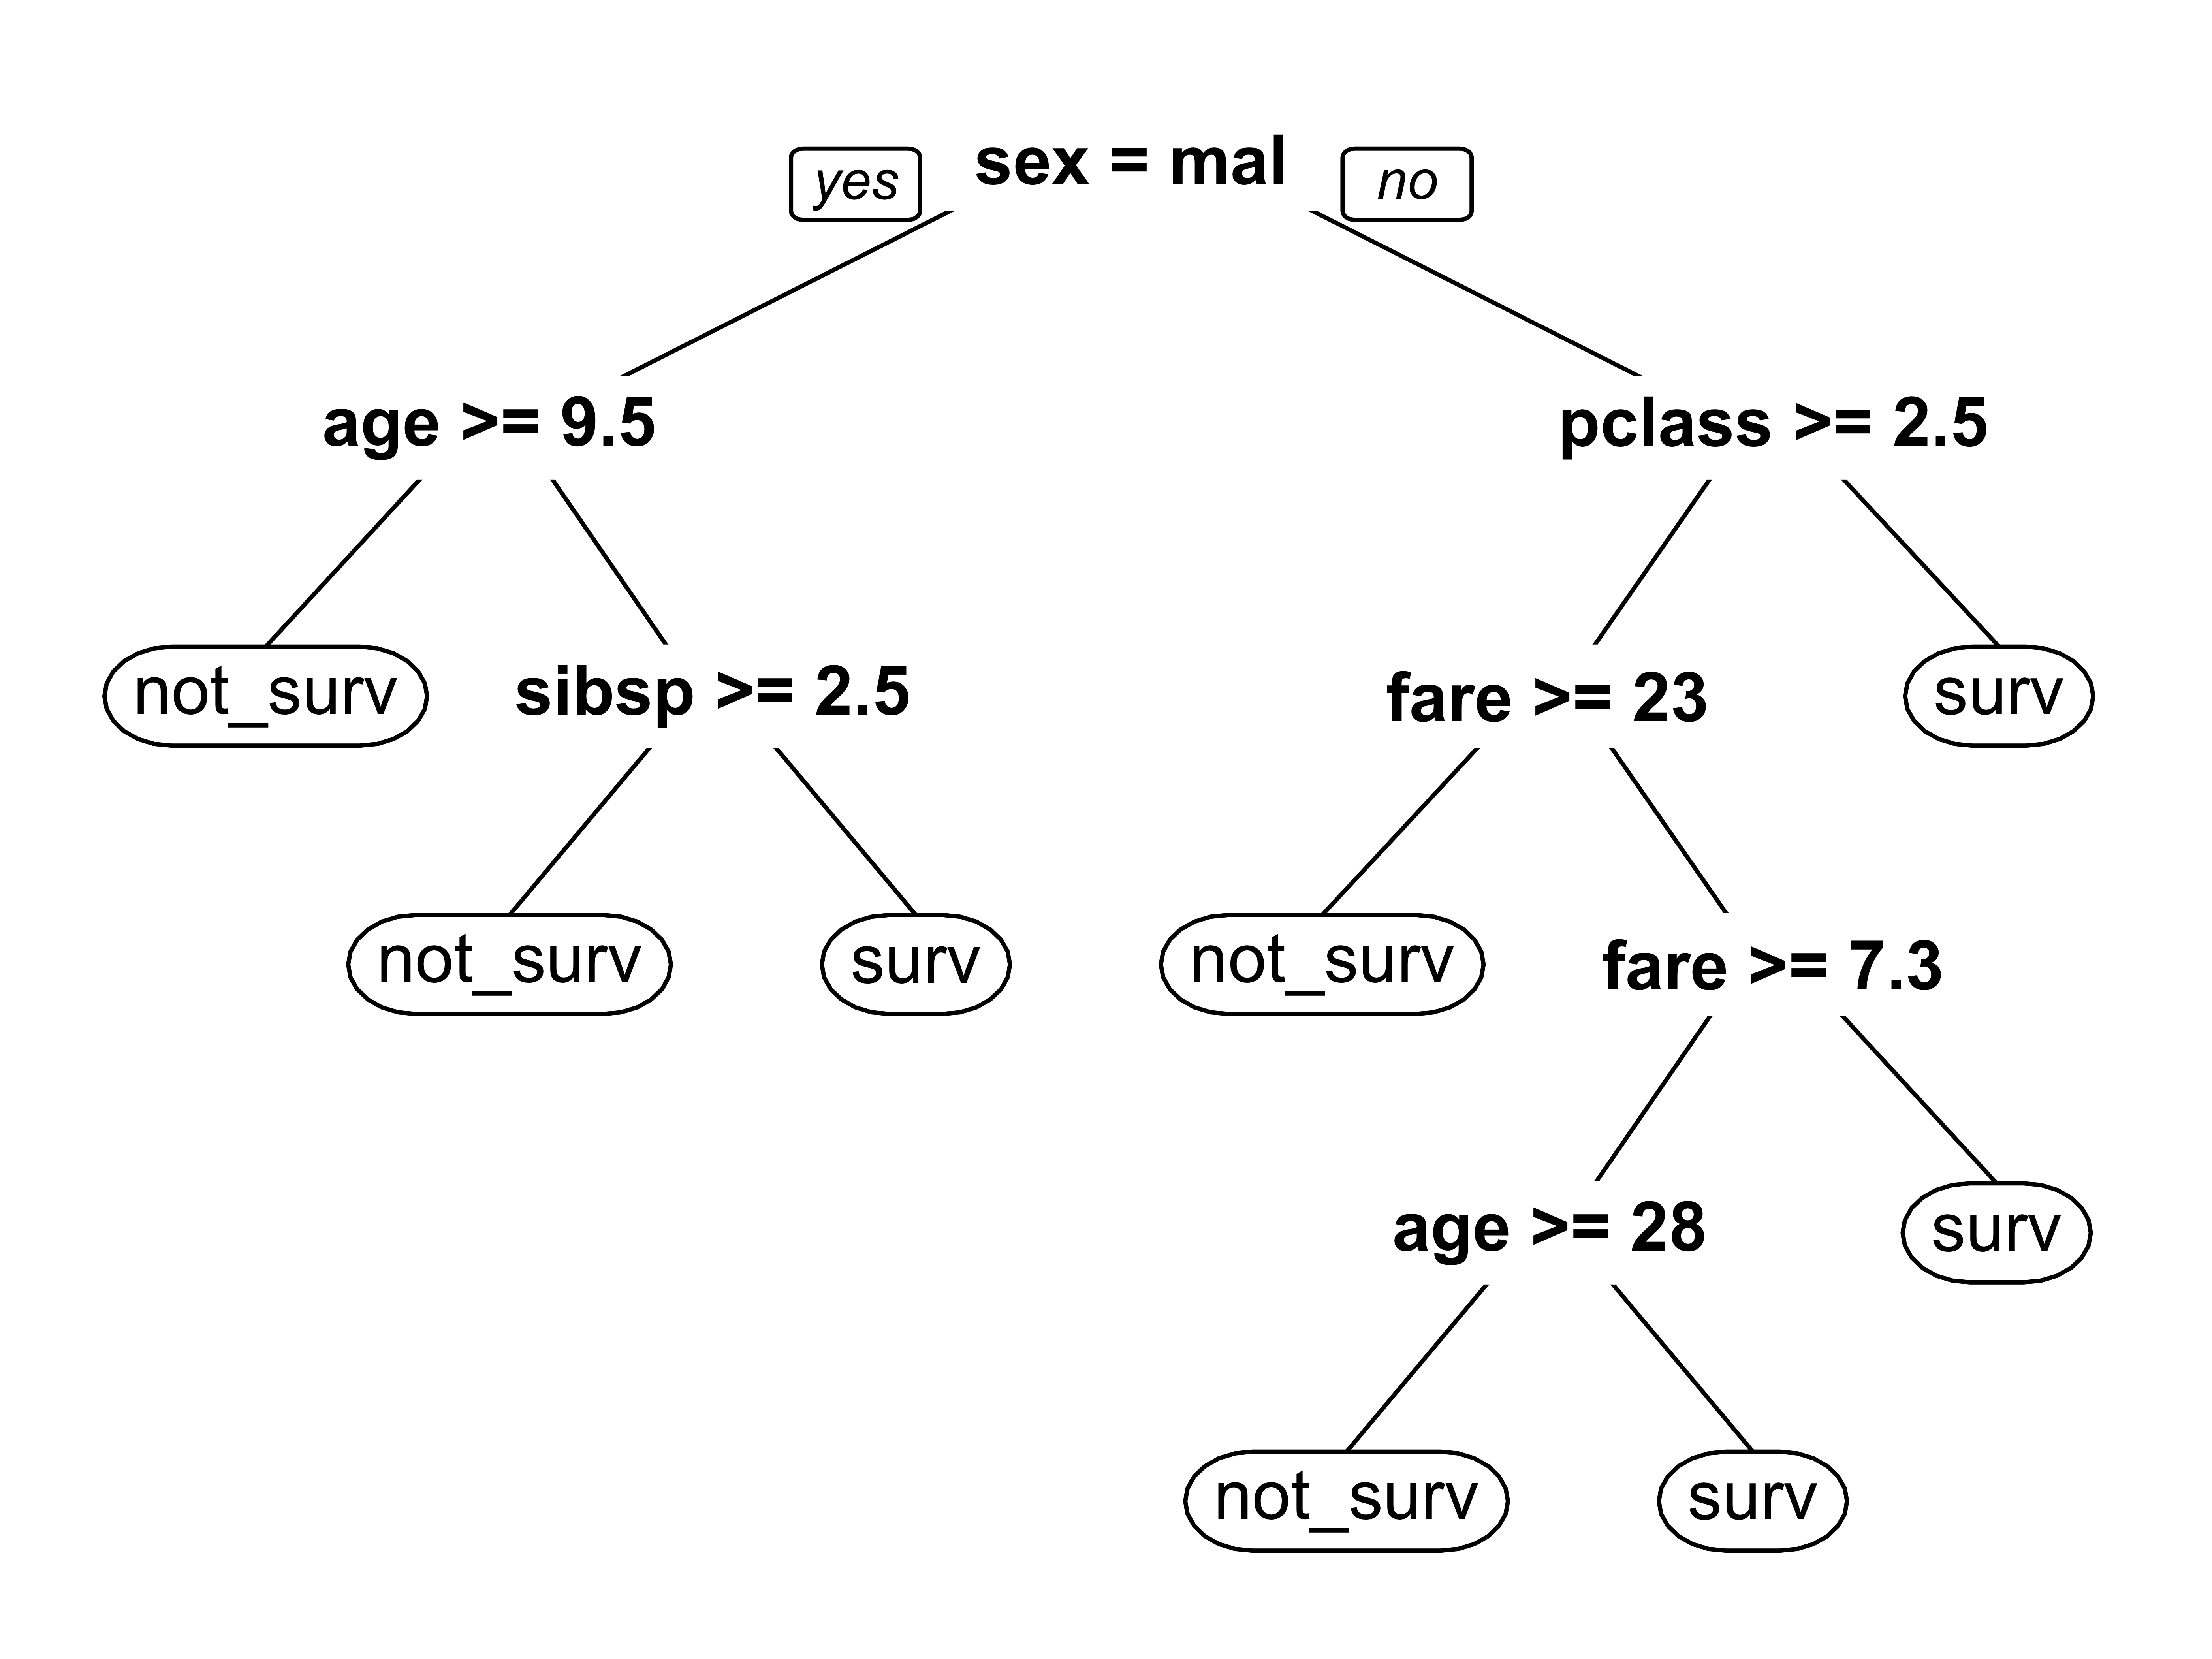
\includegraphics[scale = 0.05]{tree.png}
			\end{figure}		
    		\end{frame}

	
		\begin{frame}{Advantages of Trees-Based Methods}
			\begin{enumerate}
				\item Intuitive
				\item Viable when $n \ll p$
				\item Handle interactions naturally
				\item Minimal assumptions
				\item Handle missingness in predictors (or ``features'' for Andras \smiley)
			\end{enumerate}
		\end{frame}
	
	
	\subsection{Disadvantages of Trees}
		
		\begin{frame}{Disadvantages of Single Trees}
			\begin{enumerate}
				\item High variance
				\item Prone to overfitting
				\item Lack of smoothness (troubling for regression)
			\end{enumerate}
		\end{frame}
		
	\subsection{Bagging}
		\begin{frame}{Bootstrap Aggregation (Bagging)}
			\begin{enumerate}
				\item Breiman (1996)
				\item Extends idea of CART models
					\begin{enumerate}[1]
						\item Single trees overfit
						\item Stopping rules and pruning help, but only to a point
					\end{enumerate}
				\item Take $B$ bootstrap samples, build $B$ trees, aggregate predictions
					\begin{enumerate}[1]
						\item For regression, aggregation is taking the mean of the predicted values for each $y_i$
						\item For classification, to aggregate means each tree casts a ``vote'' for each $y_i$
					\end{enumerate}
			\end{enumerate}
    		\end{frame}
	
		\begin{frame}{Bootstrap Samples}
		$x := [1, 5, 3, 7, 9]$
		\begin{table}
		\begin{tabular}{c c c}
			\hline
			$B^{*1}$	& $B^{*2}$& $B^{*3}$  \\
			\hline
			$3$ 	& $7$ 	& $5$  \\
			$1$ 	& $1$ 	& $3$ \\
			$9$	& $7$	& $1$ \\
			$5$ 	& $3$ 	& $9$ \\
			$9$	& $1$	& $1$ \\
			\hline
		\end{tabular}
		\end{table}
		\end{frame}
		
		
		\begin{frame}{Bagging Pseudocode}
			\begin{enumerate}[]
				{\fontfamily{cmr}\selectfont
				\item{\textbf{for} $b = 1:B$}
					\begin{enumerate}[]
						\item{\hspace{3 mm} Sample random $N$ records with replacement}
						\item{\hspace{3 mm} Fit classification (or regression) tree using CART}
						\item{\hspace{3 mm} Add $b^{th}$ tree to ensemble}
					\end{enumerate}
				\item{\textbf{end}}
				\item Aggregate predictions for input $\textbf{X}$
				}
			\end{enumerate}
		\end{frame}
	
		
		\begin{frame}{Advantages of Bagging}
			\begin{enumerate}
				\item Big improvement in predictive performance
				\item Variance decreases
				\item Easy to tune
				\item Embarrassingly parallel
				\item Out-of-bag (OOB) error estimate (more on this later)
					
			\end{enumerate}
		\end{frame}

		
	
\section{Definition}
	\subsection{Random Forests}
		\begin{frame}{Random Forests}
    			\begin{enumerate}
				\item{Ho (1995), Breiman (2001)}
				\item{Extends idea of bagging}
				\item{Build many trees, aggregate predictions}
				\item{Only consider $m$ predictors at each node}
				\item{Improve predictive performance}
					\begin{enumerate}[1]
						\item Reduce inter-tree correlation
						\item Further reduce variance beyond bagging
					\end{enumerate}
			\end{enumerate}
    		\end{frame}

	\begin{frame}{Random Forest Pseudocode}
		\begin{enumerate}[]
			{\fontfamily{cmr}\selectfont
			\item{\textbf{for} $b = 1:B$}
				\begin{enumerate}[  ]
					\item{\hspace{3 mm} Sample random $N$ records with replacement}
					\item{\hspace{3 mm} Select $m$ predictors from complete set of $p$ predictors}
					\item{\hspace{3 mm} Fit classification (or regression) tree, using only $m$ predictors}
					\item{\hspace{3 mm} Add $b^{th}$ tree to ensemble}
				\end{enumerate}
			\item{\textbf{end}}
			\item{Aggregate predictions for input $\textbf{X}$}
			}
		\end{enumerate}
	\end{frame}
	

\section{Details}
	\subsection{Out-of-Bag Samples}
		\begin{frame}{OOB Samples}
		
			{\fontfamily{cmr}\selectfont
			``\textit{For each observation $z_i = (x_i, y_i)$, construct its random forest predictor by averaging \textbf{only} those trees corresponding to bootstrap samples in which $z_i$ \textbf{did not} appear.} (Hastie \textit{et al.} p. 593, 2009)''
			}
		\end{frame}
		
		\begin{frame} {OOB Samples cont.}
		In summary: \\
			\begin{enumerate}
				\item For each bootstrap iteration, we have some $(y_i, x_i)$  that weren't used in tree building
				\item Use these $(y_i, x_i)$ OOB samples to estimate test error
				\item Also use these $(y_i, x_i)$ to generate measures of variable importance (more on this later)
			\end{enumerate}
		\end{frame}
		
		\begin{frame}{OOB Error and Test Error}
			\begin{figure}
				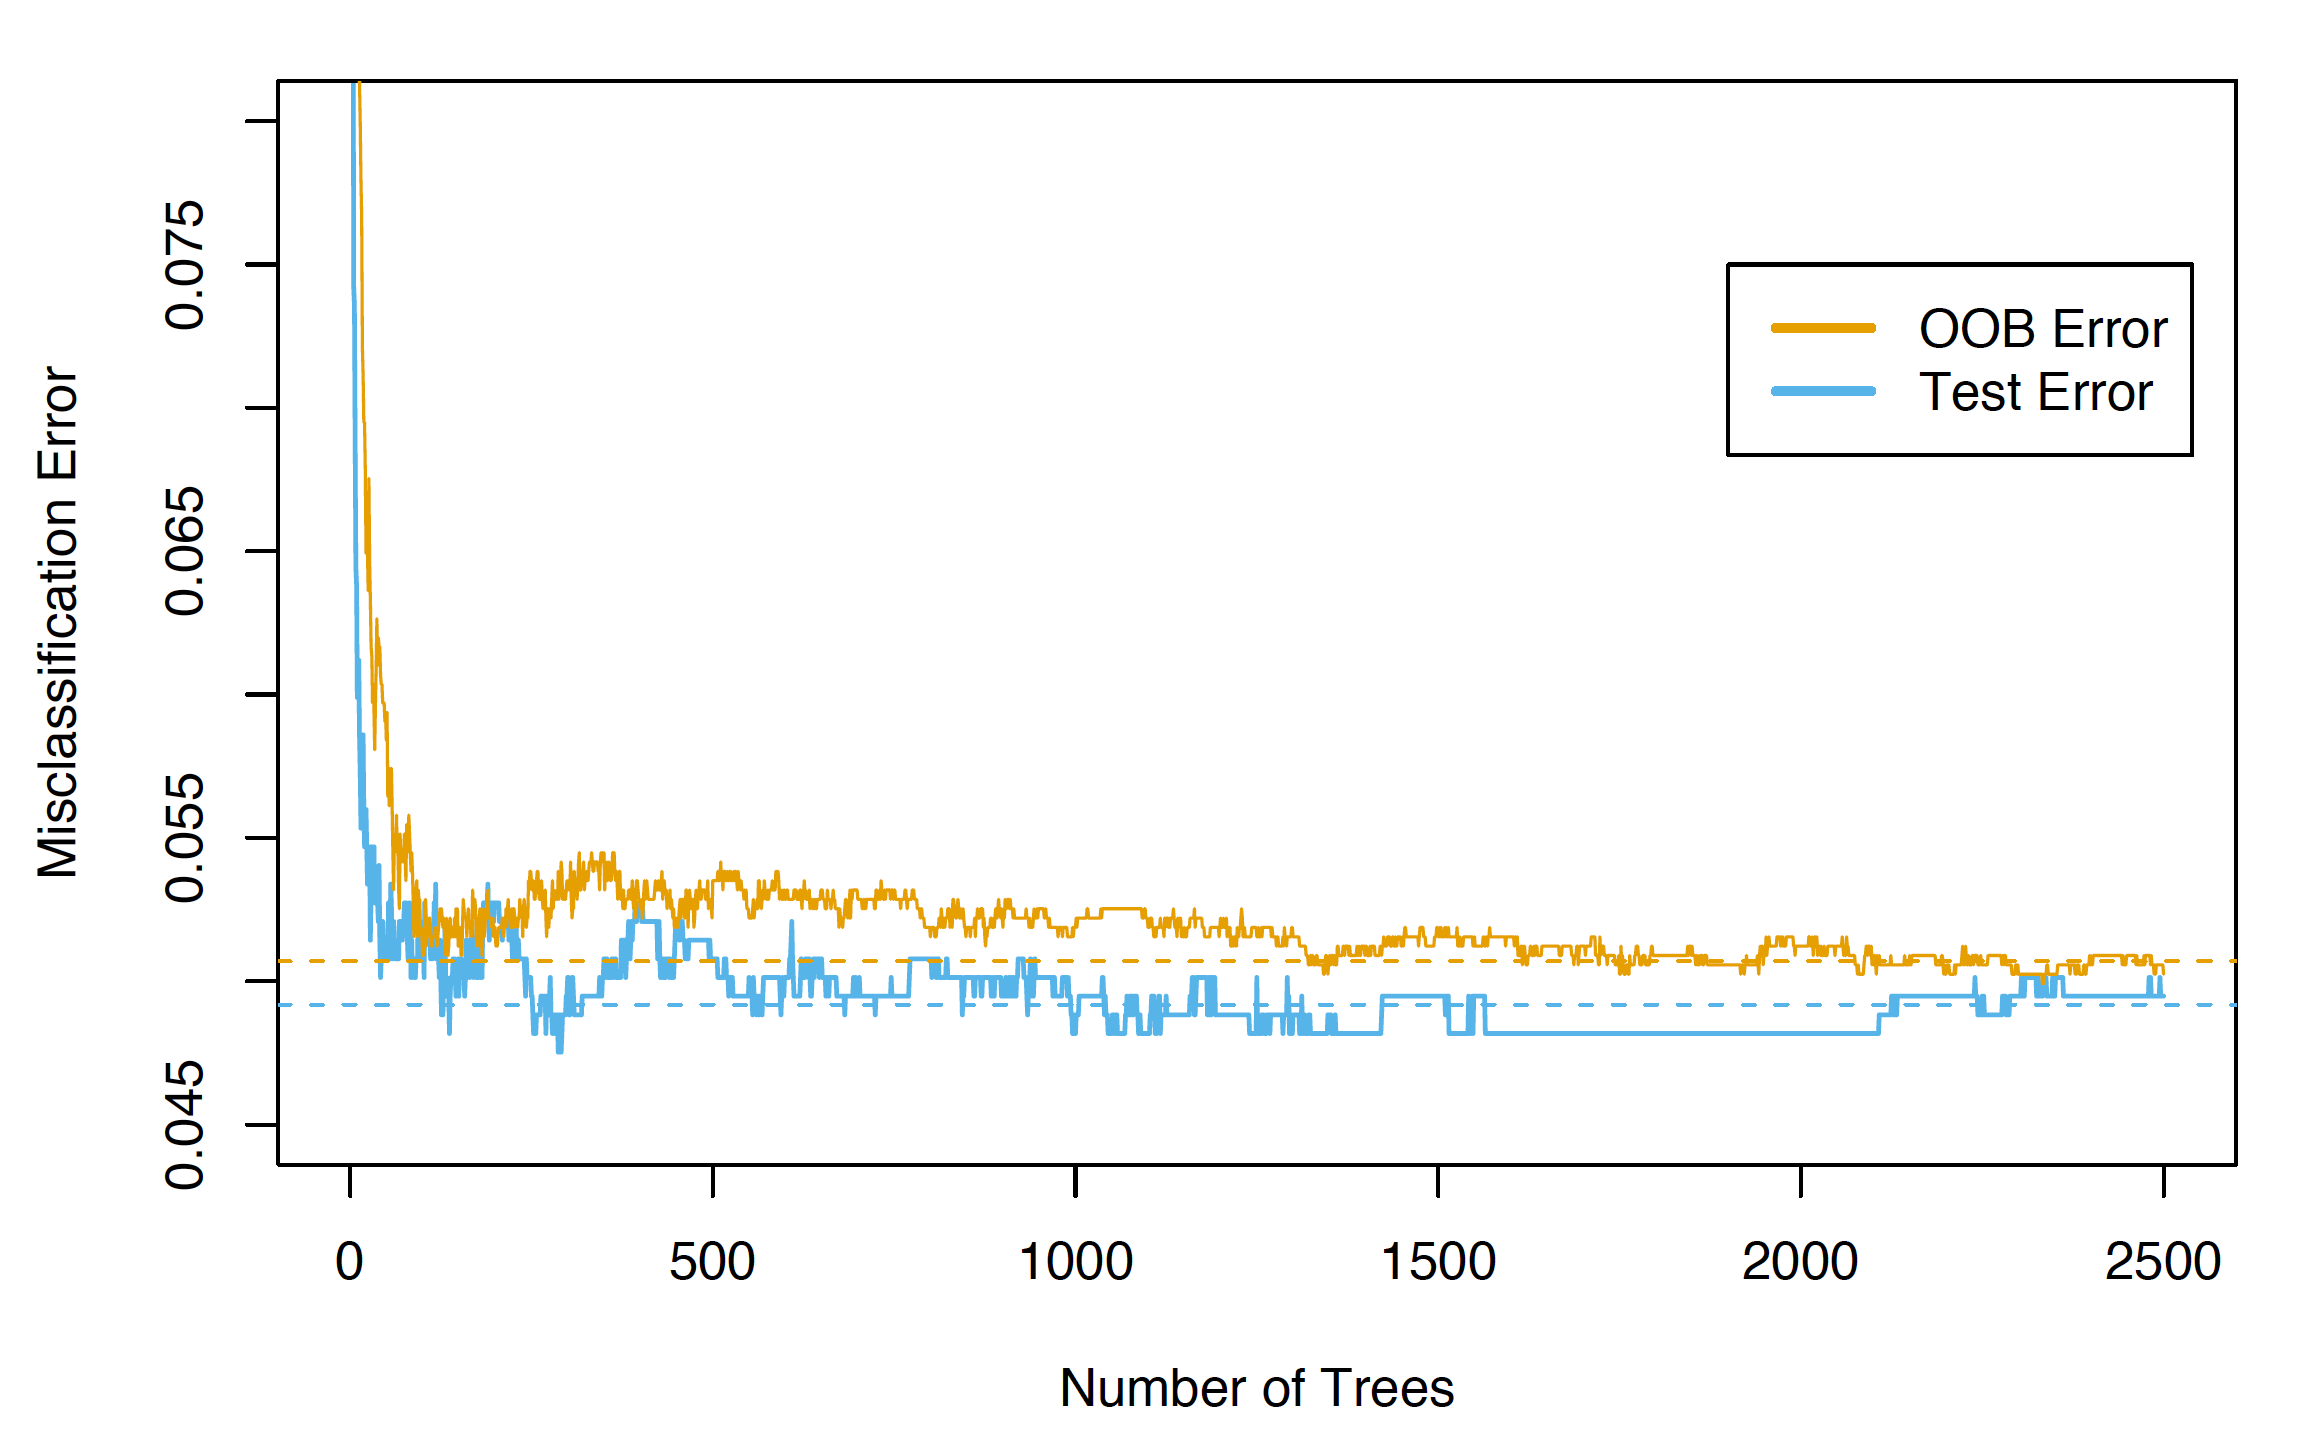
\includegraphics[scale = 0.25]{oob_error.png}
			\end{figure}		
    		\end{frame}
		
		
	\subsection{Variable Importance}
		\begin{frame}{Variable Importance}
			Variable importance computed using OOB samples:
			
			
			\begin{enumerate} [  1.]
				\item Fit $b^{th}$ tree
				\item Record prediction accuracy for OOB samples (or MSE in regression)
				\item Shuffle the $x_i$ in OOB samples
				\item Compute decrease in prediction accuracy
			\end{enumerate}
		\end{frame}
		





\section{Analysis}

	\subsection{Random Forests and Overfitting}
	
		\begin{frame}{Overfitting}
			\begin{enumerate}
				\item It was once (mistakenly) believed that random forests would not over fit
				\item You \textit{can} overfit by growing deep trees
				\item Growing too many trees won't cause you to overfit (but it's wasteful of computing resources)
			\end{enumerate}
		\end{frame}
		
		\begin{frame}{Tree Depth}
			Tree depth can be controlled in two ways:
			\vspace{5 mm}
			\begin{enumerate}
				\item{Set max number of terminal nodes (or interaction depth)}
					\begin{itemize}
						\item{\texttt{maxnodes} parameter in R}
						\item In scikit-learn, \texttt{max\char`_depth} 
					\end{itemize}
				
				\item{Specifying minimum number of observations in a node}
					\begin{itemize}
						\item{\texttt{nodesize} parameter in R}
						\item{In scikit-learn,  \texttt{min\char`_samples\char`_split}}
					\end{itemize}
			\end{enumerate}
		\end{frame}
	
	
		
\section{Conclusion}	
	
	\subsection{Advantages and Disadvantages}
		\begin{frame}{Advantages of Random Forests}
			\begin{enumerate}
				\item Powerful prediction models
				\item Easy to tune
				\item Difficult to overfit (more trees won't overfit)
				\item Variable importance
				\item Embarrassingly parallel (unlike boosting)
				\item Out-of-bag (OOB) error estimate
					\begin{enumerate}[1]
						\item Excellent approximate of test error
						\item No need for cross validation*
					\end{enumerate}

			\end{enumerate}
		\end{frame}

		\begin{frame}{Disadvantages of Random Forests}
			\begin{enumerate}
				\item Viewed as ``black box'' approach
				\item Variable importance must be interpretted cautiously
					\begin{itemize}
						\item Less interpretable than parameter estimates in parametric models
						\item Cannot meaningfully compare random forest to boosting 
					\end{itemize}  
				\item Trouble predicting severe outliers
					\begin{itemize}
						\item In regression, training data constrains the max (or min) $\hat{y}_i$ values 
						\item In parametric models, the $\hat{y}_i$ values aren't bounded in this way
					\end{itemize}
				
			\end{enumerate}
		\end{frame}
	
	\subsection{Other Remarks}
		\begin{frame}{Other Remarks}
			\begin{enumerate}
				\item In very noisy data, \texttt{mtry} parameter (in R) or \texttt{max\char`_features} (in scikit-learn) should be set higher
				\item Often, boosting will tend to \textit{slightly} outperform random forests
					\begin{itemize}
						\item This is very case-specific, however
						\item Boosting will tend to have the advantage in very noisy data
					\end{itemize}
				
			\end{enumerate}
		\end{frame}
		
	\begin{frame}{\hspace{3 mm}}
		\begin{center}
			Thank you!
		\end{center}
	\end{frame} 
		
		
		
\end{document}